\title{INF569 Project report}
\documentclass[paper=a4, fontsize=11pt]{scrartcl}
\usepackage[T1]{fontenc}
\usepackage{fourier}

\usepackage[english]{babel}
\usepackage[protrusion=true,expansion=true]{microtype}	
\usepackage{amsmath,amsfonts,amsthm}
\usepackage{hyperref}
\usepackage{minted}
\usepackage{graphicx}

\usepackage{sectsty}
\allsectionsfont{\centering \normalfont\scshape}

\usepackage[nottoc, notlof, notlot]{tocbibind}

\usepackage{fancyhdr}
\pagestyle{fancyplain}
\fancyhead{}											% No page header
\fancyfoot[L]{}											% Empty 
\fancyfoot[C]{}											% Empty
\fancyfoot[R]{\thepage}									% Pagenumbering
\renewcommand{\headrulewidth}{0pt}			% Remove header underlines
\renewcommand{\footrulewidth}{0pt}				% Remove footer underlines
\setlength{\headheight}{13.6pt}

\numberwithin{figure}{section}			% Figurenumbering: section.fig#
\numberwithin{table}{section}				% Tablenumbering: section.tab#

\newcommand{\horrule}[1]{\rule{\linewidth}{#1}} 	% Horizontal rule

\title{	
		\usefont{OT1}{bch}{b}{n}
		\normalfont \normalsize \textsc{INF569: Modeling and Analysis of \\ Cyber-Physical Systems} \\ [25pt]
		\horrule{0.5pt} \\[0.4cm]
		\huge Intelligent traffic lights controller \\
		\horrule{2pt} \\[0.5cm]
}
\author{
		\normalfont 								\normalsize
        Lo\"{i}c Gelle\\[-3pt]		\normalsize
        \today
}
\date{}


%%% Begin document
\begin{document}
\maketitle
\section{Introduction}

The increasing number of vehicles in urban areas triggers major traffic congestion problems every day. Added to a general lack of comfort of the individuals are the more global problems of road management, like handling emergency vehicles stuck in the middle of the traffic. The existing methods of traffic management are inadequate both during peak hours, when traffic lights are incapable of getting the maximal throughput of vehicles, and during off-peak times when people can get stuck at a red light during a few minutes although no one else is waiting at the crossroads. In this context, it is critical to be able to design traffic lights controllers that adapt to both situations to minimize individual discomfort and to optimize road use. Related works saw the light of day quite recently, for example in Copenhagen where intelligent traffic lights prioritize bus and bicycles over cars, showing that the subject is both intricate and a burning issue.\\

The aim of this project is to propose and analyse a simple model of traffic lights controller to address these problems. This will be done using Stateflow and under the assumption that we only consider a single intersection between two roads. In particular, communication between several such controllers will not be addressed in the implementation.

\section{System notations and specification}

Let us consider an intersection such as described in figure \ref{intersection}. It is composed of four incoming directions -- N for North, E for East, S for South and W for West -- each of which having three incoming lanes: the leftmost one for people willing to turn left, the rightmost one for people willing to turn right and the last one for people going straight ahead.

\begin{figure}[!ht]
    \center
    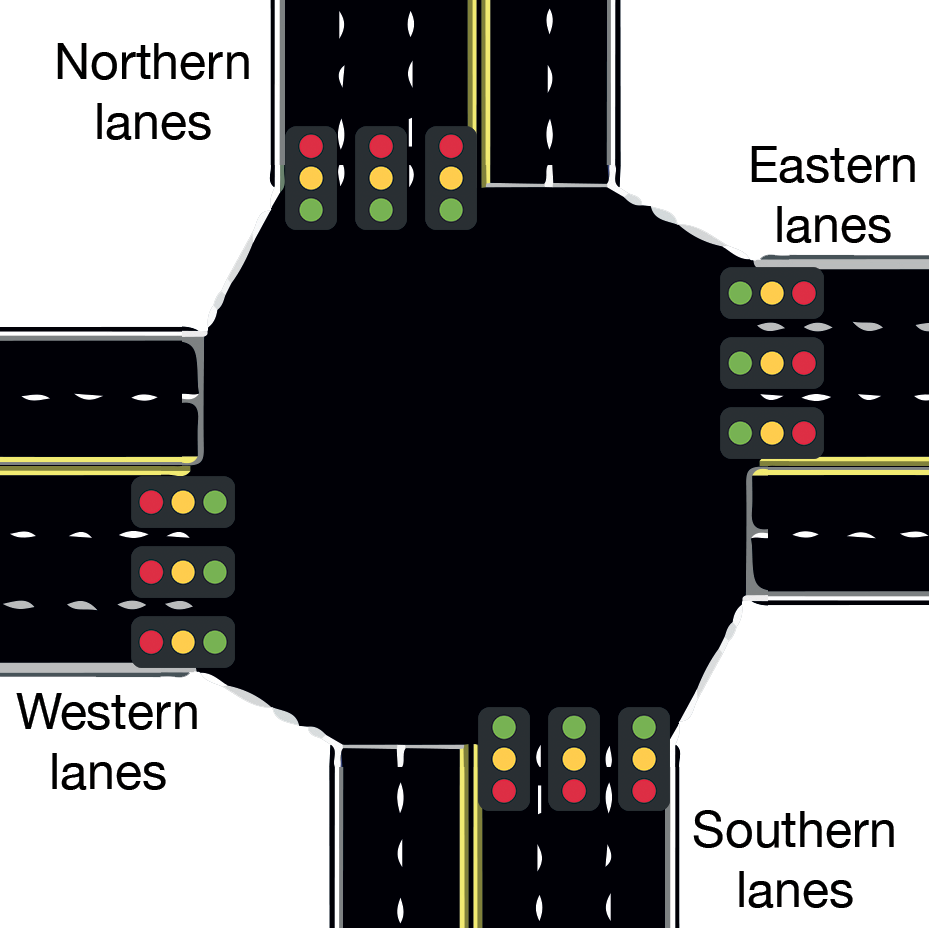
\includegraphics[width=0.4\textwidth]{./images/intersection.png}
    \caption{\label{intersection} The intersection considered.}
\end{figure}

We make the assumption that each of the four directions have its own traffic light, its own incoming flow meter and its own queue of waiting vehicles. We can build 11 optimized phases based on these informations, all described in figure \ref{possibilities}.

\begin{figure}[!ht]
    \center
    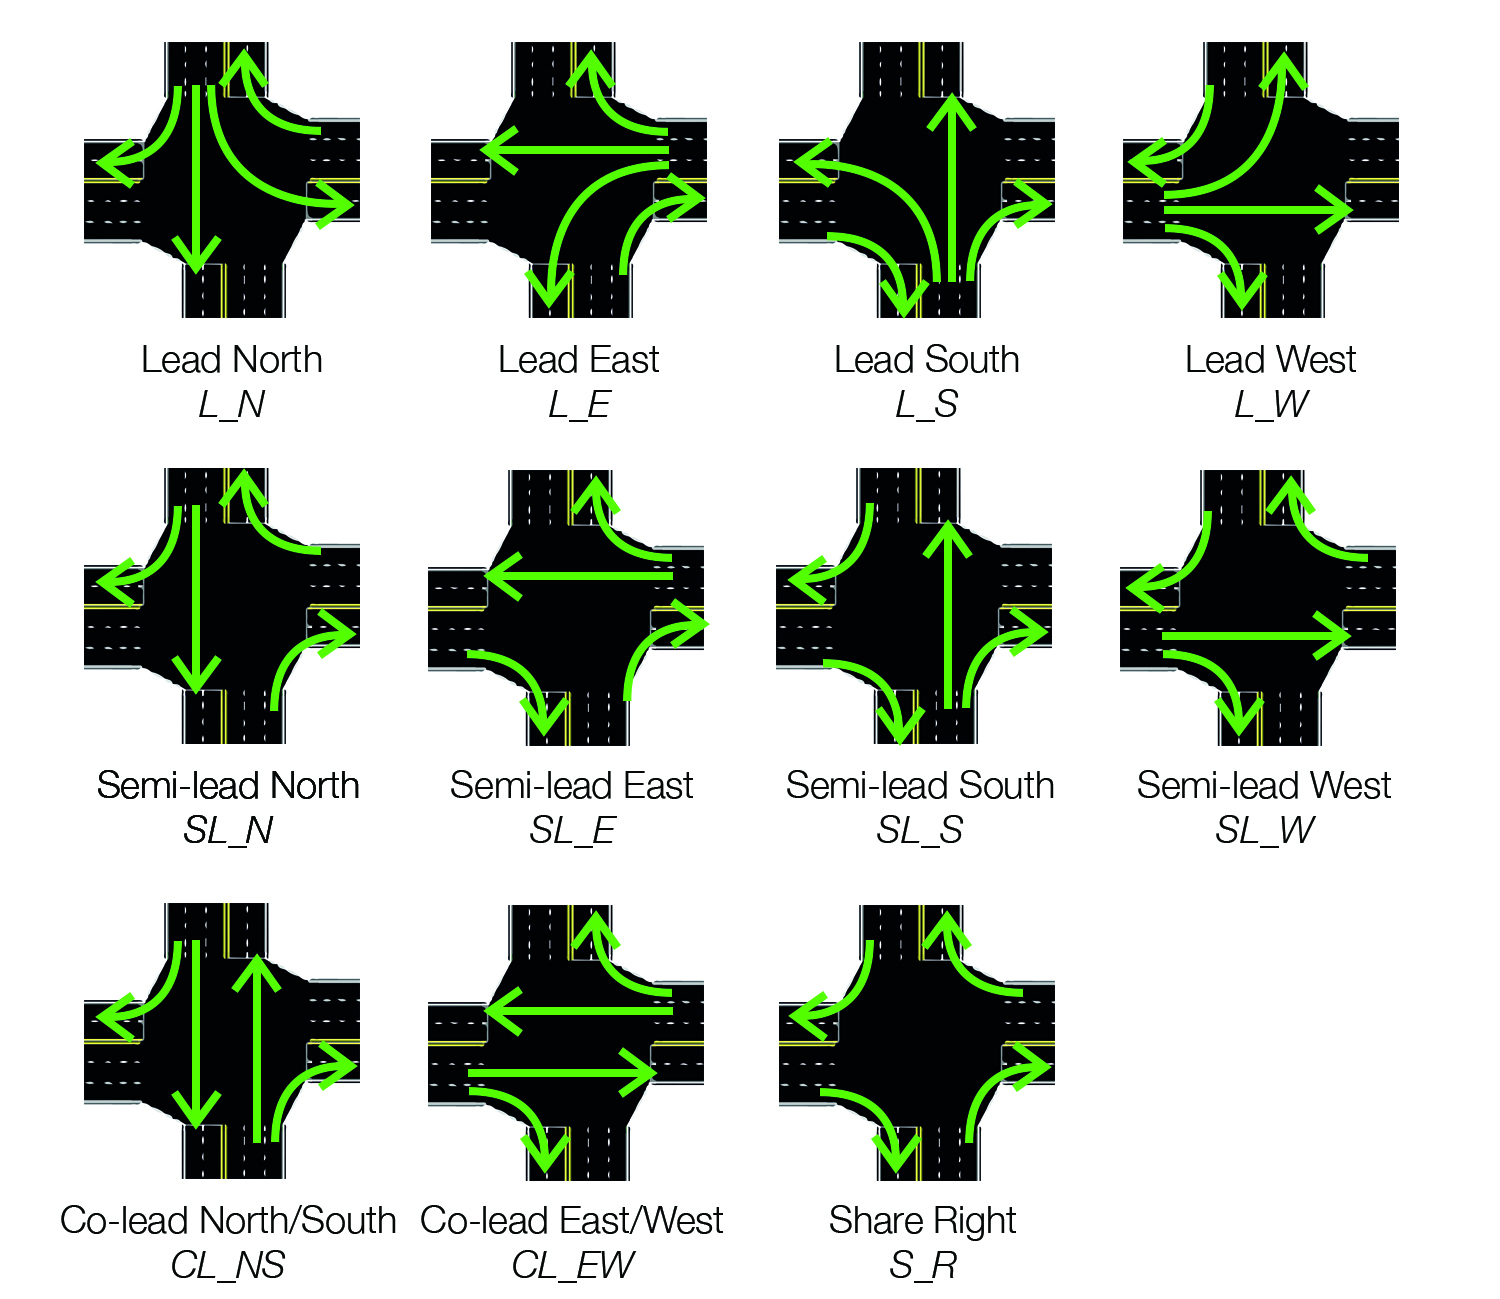
\includegraphics[width=0.7\textwidth]{./images/possibilities.jpg}
    \caption{\label{possibilities} The possible phases.}
\end{figure}

Informally, we expect a model that is specified thus:
\begin{itemize}
\item Each of the lanes has to be given a "fair" passing time, using these 11 phases;
\item No one waits indefinitely in a lane;
\item Queue sizes are always positive;
\item The controller prevents impossible combinations of green lights
\item No vehicle should be waiting if all the other lanes are empty
\item No Zeno behaviour shall be observed.
\end{itemize}

The design of the model intents to address these specifications, that will not be formally verified by lack of time and tools. Nonetheless, ideas on how to verify them will be given in the following sections.

\section{Model proposed}

The idea is to give each of the phases a coefficient that is a linear combination of the sizes of the queues that are involved. The coefficient of the phase "Lead North" will be:

\[
c_{L\_N} = 3 q_{N\_R} + 7 q_{N\_S} + 21 q_{N\_L} + 3 q_{E\_R}
\]

where the variable \(q_{N\_S}\) represents the queue size of the vehicles coming from North and going straight ahead. The coefficient of the combination are chosen in a way that balances the number of occurences of each direction in the phases; actually, "turning right" from a given direction occurs in 7 phases, while "turning left" from that same direction only occurs once and "going straight ahead" occurs 3 times. It is important to notice that, for the sake of simplicity, the queue sizes are real numbers and not natural numbers.\\

The phases will be consecutive, and the passing time of the current phase right before it begins. For the example phase, that gives us:

\[
d_{L\_N} = \text{min}\left(\dfrac{c_{L\_N}}{\sum_{p \in Phases} c_p} cycle\_duration, max\_phase\_duration\right)
\]

where \(cycle\_duration\) is a -- fixed -- rough estimate of the time given to all phases, and \(max\_phase\_duration\) prevents the intersection to be monopolized by a single phase.\\

The main controller of the stateflow model implements this idea, using a simple Matlab function \texttt{computeTimes} that is defined thus:

\begin{minted}{matlab}
function computeTimes

q_sum_L_N = 3 * q_N_R + 7 * q_N_S + 21 * q_N_L + 3 * q_E_R;
\% define other coefficients the same way
\% (...)

q_sum = q_sum_L_N + q_sum_L_E + q_sum_L_S + q_sum_L_W
	+ q_sum_CL_NS + q_sum_CL_EW + q_sum_SL_N + q_sum_SL_E
	+ q_sum_SL_S + q_sum_SL_W + q_sum_S_R;

if (q_sum <= 0)
    d_L_N = 0;
    \% define other durations the same way
    \% (...)
else
    d_L_N = min(q_sum_L_N * cycle_duration / q_sum, max_phase_duration);
    \% define other durations the same way
    \% (...)
end
\end{minted}

A part of the controller is shown in figure \ref{model_1}.

\begin{figure}[!ht]
    \center
    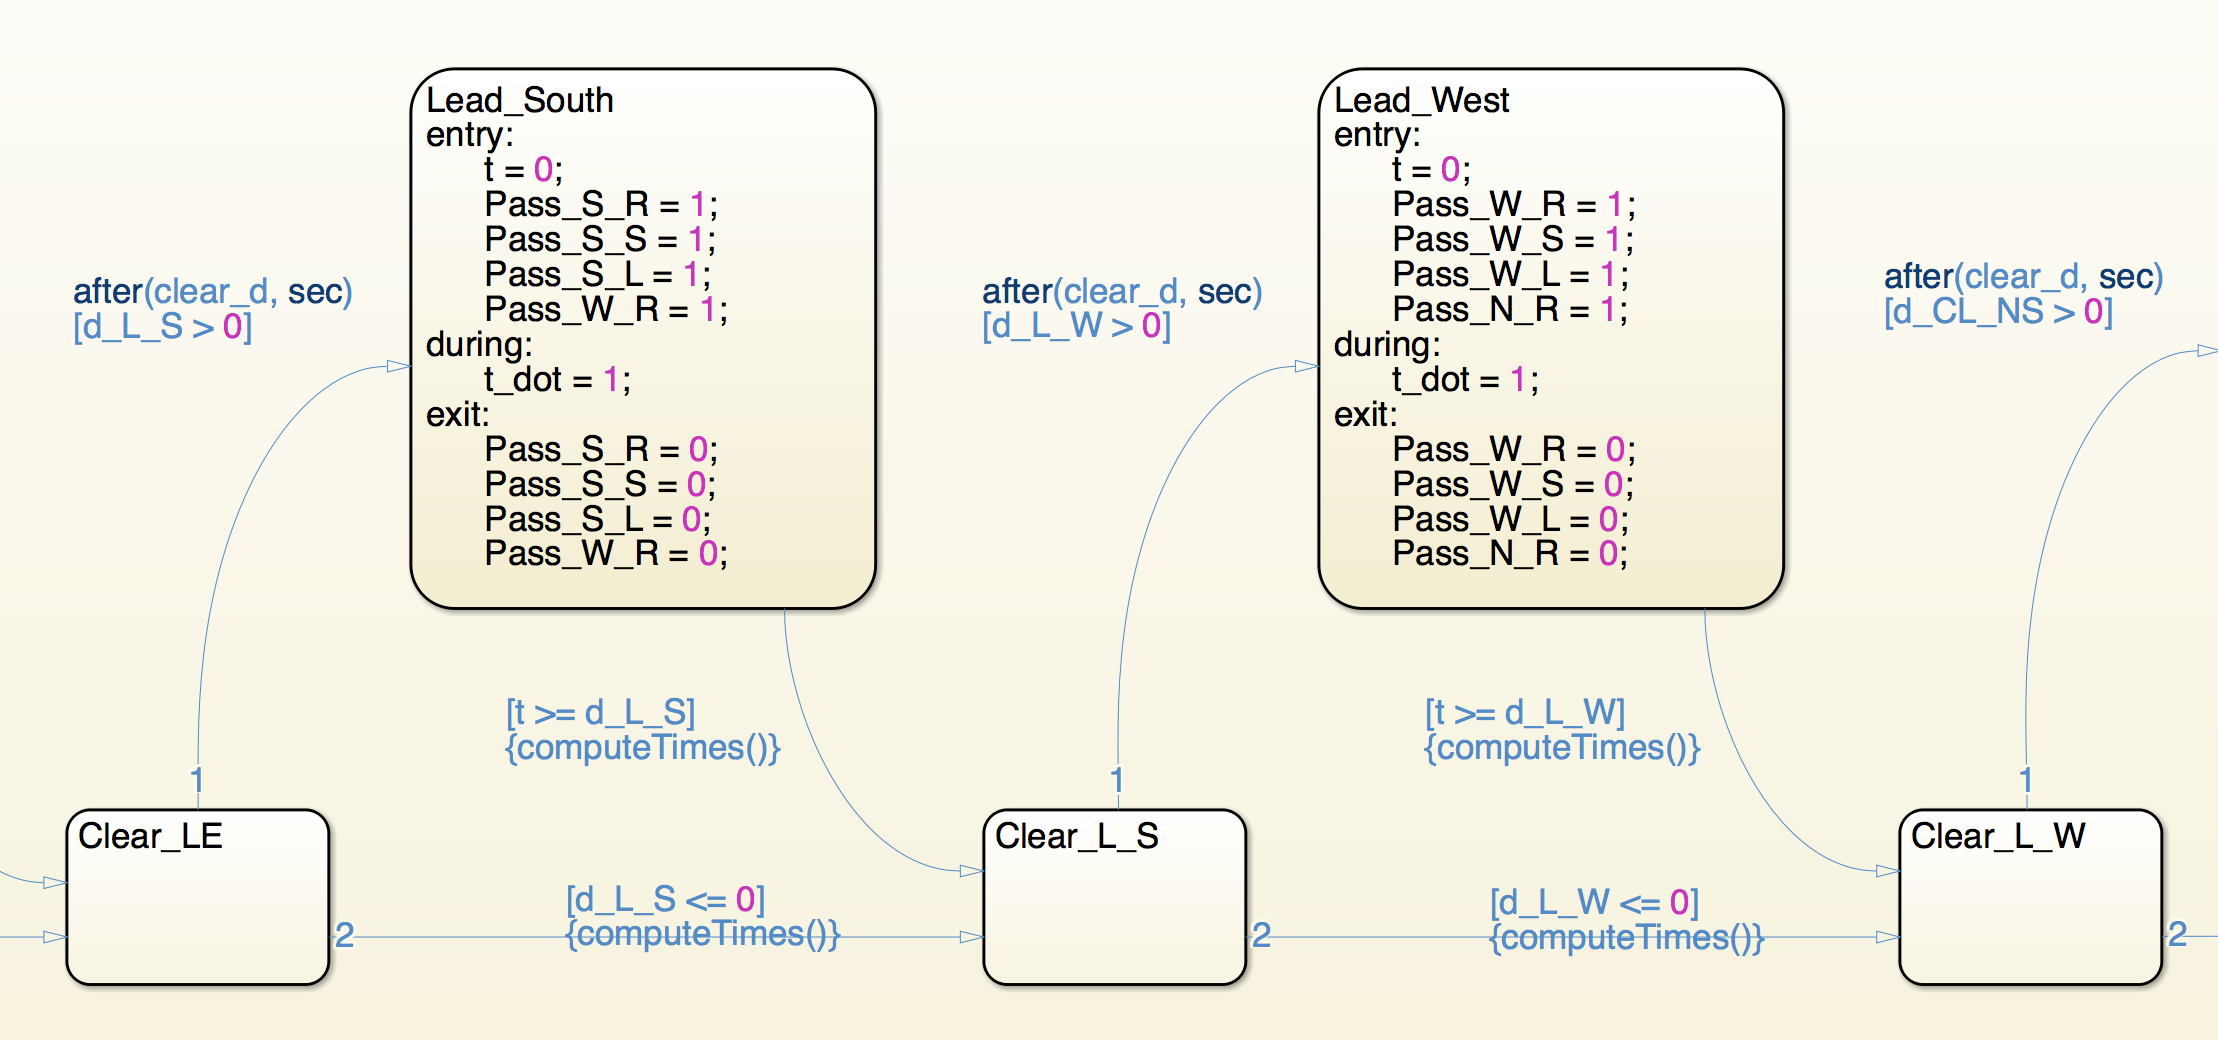
\includegraphics[width=1\textwidth]{./images/model_1.png}
    \caption{\label{model_1} The control flow of the model.}
\end{figure}

In the model, every phase is followed by a clearance period during which no light is green. This succession of cleared states allows the controller to jump immediately to the next phase that is granted a non-zero duration. Each lanes has its own queue handler that ensures that queue sizes are non-negative and evolve according to the corresponding light state -- see figure \ref{model_2}.

\begin{figure}[!ht]
    \center
    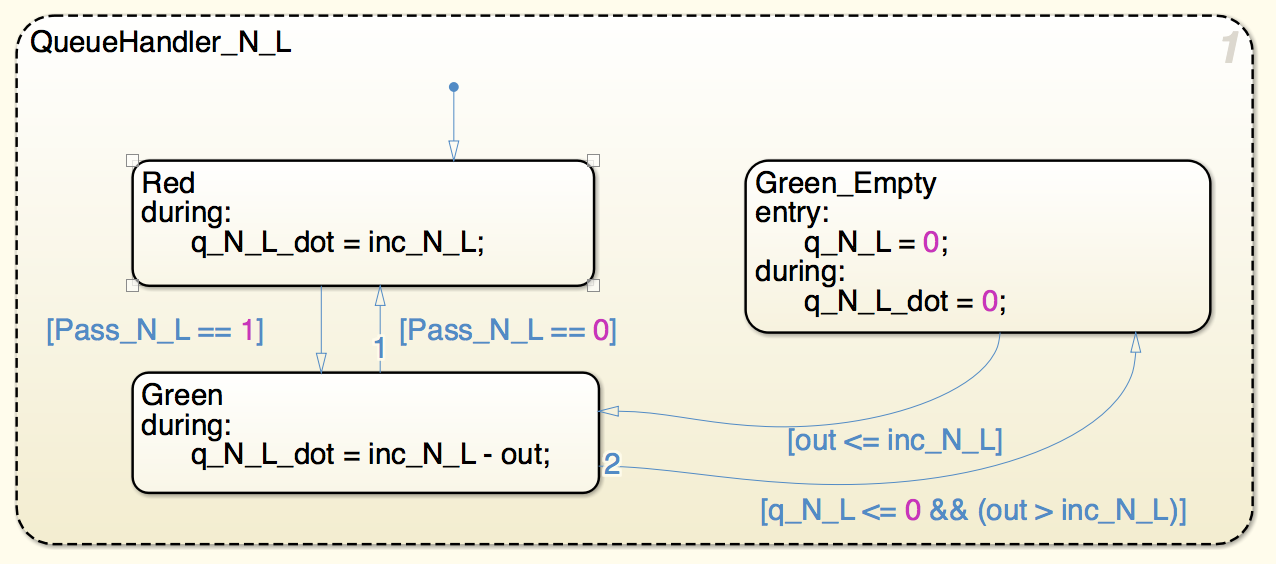
\includegraphics[width=0.8\textwidth]{./images/model_2.png}
    \caption{\label{model_2} A queue handler in the model.}
\end{figure}

The Simulink model allows the user to specify the inputs -- such as the incoming flow of vehicles for each direction or the cycle duration -- and to observe visually the evolution of the system.

\section{Simulation and verification methods}

The specified properties could not be formally verified using appropriate tools. They were manually checked using specific case simulations and showed that the model globally behaves as expected. In particular, the controller never triggers dangerous green light combinations -- essentially by design -- and seems to balance passing times according to queue sizes. The Zeno and queue signs problems were anticipated by design, with a fixed waiting time after a complete loop of clearance states and an appropriate state in the queue handlers.\\

More advanced simulations would have required real-life and usable data, but what I found on the Internet was charged. Nevertheless, as for verification properties, we can think of a way things would have been done with more time and the appropriate tools. The following subsections try to give methods and ideas.\\

\subsection{Drivers satisfaction}

The desired properties of fair passing times and reduced waiting times are key. Studies and benchmarks are necessary to ensure them. What I would propose is to slightly change the data structure of the queue sizes in order to keep track of the waiting times. Actually, a simple queue size cannot give enough information to answer those questions of type : "since when is vehicle A waiting in this lane?" or "how many people have been waiting here for more than x seconds?".\\

One solution would be to replace the queue size by an infinite vector

\[
q = (q_0, q_1, ..., q_i, ...)
\]

where \(q_i\) represents the number of vehicles that have been waiting for \(t \in \mathopen{[}i, i+1\mathclose{]}\) time units. This could be handled easily in any sound programming language, but could be problematic in Matlab.\\

The second solution would be to replace the queue size by a pair \(n, m\) where \(n\) represents the number of vehicles waiting and \(m\) the average waiting time. This pair gives less information than the previous vector, but could be easily updated in well-chosen Stateflow states.

\subsection{Zeno behaviour}

Another challenge is to prove that our system will never get stuck in a Zeno behaviour in which the time does not pass no more. This could be done by adding a subsystem that has its own clock and that checks every time unit that the time has actually passed. If not, the subsystem would enter in an error state that could be detected by a reachability analysis.

\subsection{Security concerns}

The main security issue would be to have two conflicting lights being activated at the same time. An appropriate reachability analysis could prove the system secure, if we define for example a subsystem that enters an error state in case of inconsistent combination.\\

Another solution would be to describe all conflicting combinations in a boolean logic formula, and ensure by analysis that this formula never happens to be true.

\section{Going further}

The main drawback of the implemented model is that there is no state that really "takes a decision", as the control flow is quite decentralized. That makes it costly to modify transitions or to add a phase.\\

Refactoring the model naturally leads to a more centralized version in which a node has the responsability to call the function \texttt{computeNextState} and to switch state to the right phase. This model is implemented as well, and it is important to notice that it chooses the next phase using objective functions, and not in the same sequential order.\\

According to hand-made simulations, this new model is quite good in terms of balancing between the phases. The next step to explore would logically be the coordination between several such models in order to build intelligent and adaptative traffic light networks.

\bibliographystyle{plain}
\bibliography{biblio}
\nocite{*}

\end{document}